\subsection{Struktura wirtualnego receptora}
\label{subsec:vr-camera-struktura}

\begin{figure}[ht]
    \centering
    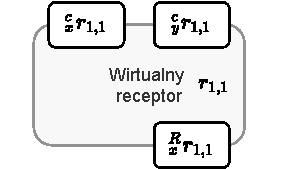
\includegraphics[width=0.75\columnwidth]{figures/ISR-vr-camera-model.pdf}
    \caption{Struktura ogólna wirtualnego receptora kamery RGB-D}
    \label{fig:model-vr-camera}
\end{figure}

Na rysunku~\ref{fig:model-vr-camera} przedstawiono strukturę wirtualnego receptora. Jego rolą jest odbiór surowych danych pomiarowych z~rzeczywistego receptora oraz ich obróbka i~agregacja przed wysłaniem ich do podsystemu sterowania. Do poprawnej pracy podsystemu, wymagane są trzy bufory komunikacyjne: dwa do komunikacji z~podsystemem sterowania oraz jeden do odbioru danych z~kamery. Krok dyskretyzacji wirtualnego receptora jest wąskim gardłem systemu. Założono że receptor jest w~stanie działać z krokiem ${}^{r}T = \frac{1}{30}$s, czyli takim z~jakim działa wirtualny receptor. Założenie to jest wykonalne z~racji niskiej rozdzielczości kamer tego typu.

\subsubsection{Bufory komunikacyjne}
\begin{itemize}
    \item ${}^{c}_{x}r_{1,1} = \varphi \in \{b, p\}$ - tryb detekcji klocków/miejsc,
    \item ${}^{c}_{y}r_{1,1} = \Theta_{d}$ - pozycja wykrywanego klocka/miejsca,
    \item ${}^{R}_{x}r_{1,1} = \Lambda$ - chmura punktów z~kamery RGB-D.
\end{itemize}

\subsubsection{Funkcje pomocnicze}
Do poprawnego działania receptora, wymagana jest implementacja kilku funkcji pomocniczych, których konkretna definicja wymaga dokładnych parametrów omawianej kamery oraz budowy palety. Ich nagłówki zostały ograniczone do minimum, tak aby przedstawić ideę przetwarzania w~podsystemie.

\begin{itemize}
    \item \texttt{detect($\Lambda$)} - wykryj żółty sześciany
    \item \texttt{getTF($c$)} - zwróć pozycję podanego sześcianu,
    
    \item \texttt{find($\Lambda$)} - wykryj możliwe położenia do odstawienia,
    \item \texttt{getFinal($s$)} - zwróć pozycję docelowych położeń do odstawienia sześcianu, wraz z~ich koordynatami na palecie.
\end{itemize}

\subsection{Automat sterujący}
\begin{figure}[ht]
    \centering
    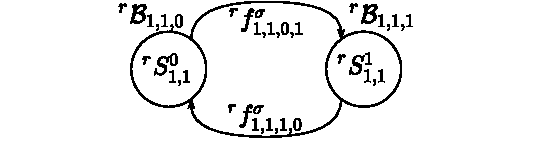
\includegraphics[width=\columnwidth]{figures/ISR-vr-camera-behaviours.pdf}
    \caption{Automat zachowań wirtualnego receptora kamery RGB-D}
    \label{fig:zachowania-vr-camera}
\end{figure}


Na rysunku~\ref{fig:zachowania-vr-camera} przedstawiony został automat sterujący wirtualnym receptorem kamery. Z~każdym z~dwóch stanów $ {}^{r}S_{1,1}^0,  {}^{r}S_{1,1}^1$ skojarzone zostało zachowanie ${}^{r}\mathcal{B}_{1,1,0}$ (\textbf{blocks}) oraz ${}^{r}\mathcal{B}_{1,1,1}$ (\textbf{places}). Każde z~zachowań określa tryb przetwarzania danych z~kamery. Wybór zachowań następuje poprzez wysłanie odpowiedniej wartości na bufor wejściowy.

\subsection{Zachowanie blocks}
\label{subsec:vr-camera-blocks}
Zachowanie ${}^{r}\mathcal{B}_{1,1,0}$ określa tryb wykrywania żółtych sześcianów. Gdy to zachowanie jest aktywne, na bufor ${}^{c}_{y}r_{1,1} = \Theta_{d}$ wysyłana jest pozycja wykrytego klocka lub wartość pusta. 

\subsubsection{Funkcja przejścia}
\begin{equation}
    {}^{r_{1,1}, c_{1,1}}f_{1,1,0} \triangleq {}^{c}_{y}e_{1,1} = \text{\texttt{getTF(detect(}}\Lambda\text{\texttt{))}}    
\end{equation}

\begin{figure}[ht]
    \centering
    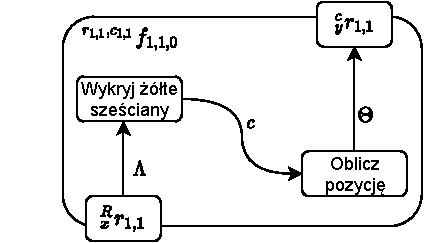
\includegraphics[width=\columnwidth]{figures/ISR-vr-camera-fp-blocks.pdf}
    \label{fig:vr-camera-fp-blocks}
    \caption{Zdekomponowana funkcja przejścia zachowania \textbf{blocks} w~postaci DFD}
\end{figure}

\subsubsection{Warunki początkowe}
\begin{equation}
    {}^{r}f^{\sigma}_{1,1,1,0} \triangleq \varphi = b
\end{equation}

\subsubsection{Warunki końcowe}
\begin{equation}
    {}^{r}f^{\tau}_{1,1,0} \triangleq \varphi \neq b
\end{equation}

\subsection{Zachowanie places}
\label{subsec:vr-camera-places}
Zachowanie ${}^{r}\mathcal{B}_{1,1,1}$ określa tryb wykrywania miejsc na palecie. Gdy to zachowanie jest aktywne, na bufor ${}^{c}_{y}r_{1,1} = \Theta_{d}$ wysyłana jest lista dostępnych pozycji wraz z~ich koordynatami na palecie lub wartość pusta. 

\subsubsection{Funkcja przejścia}
\begin{equation}
    {}^{r_{1,1}, c_{1,1}}f_{1,1,1} \triangleq {}^{c}_{y}e_{1,1} = \text{\texttt{getFinal(find(}}\Lambda\text{\texttt{))}}  
\end{equation}

\begin{figure}[ht]
    \centering
    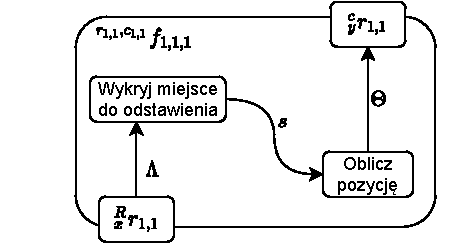
\includegraphics[width=\columnwidth]{figures/ISR-vr-camera-fp-places.pdf}
    \label{fig:vr-camera-fp-places}
    \caption{Zdekomponowana funkcja przejścia zachowania \textbf{places} w~postaci DFD}
\end{figure}

\subsubsection{Warunki początkowe}
\begin{equation}
    {}^{r}f^{\sigma}_{1,1,1,0} \triangleq \varphi = p
\end{equation}

\subsubsection{Warunki końcowe}
\begin{equation}
    {}^{r}f^{\tau}_{1,1,0} \triangleq \varphi \neq p
\end{equation}
